\label{sec:intro}


Billion-parameter generative models trained to imitate human language and behaviors from web datasets have unlocked unprecedented generality in machine learning \cite{touvron2023llama, team2023gemini}. While evaluations of these large language models (LLMs) are organized into discrete benchmarks \cite{hendrycks2020measuring} with specific themes like competitive mathematics \cite{Hendrycks2021MeasuringMP} or reading comprehension \cite{dua-etal-2019-drop}, their knowledge transfers to countless problems. LLMs' flexibility is largely due to an “in-context learning” effect that emerges when input sequences grow long enough to resemble a dataset of examples for a new task \cite{brown2020language, kirsch2022general}. However, predicting the most likely continuation of a sequence is misaligned with optimal control and limits us to tasks where high-quality demonstrations are available.

\begin{figure}[h!]
    \centering
    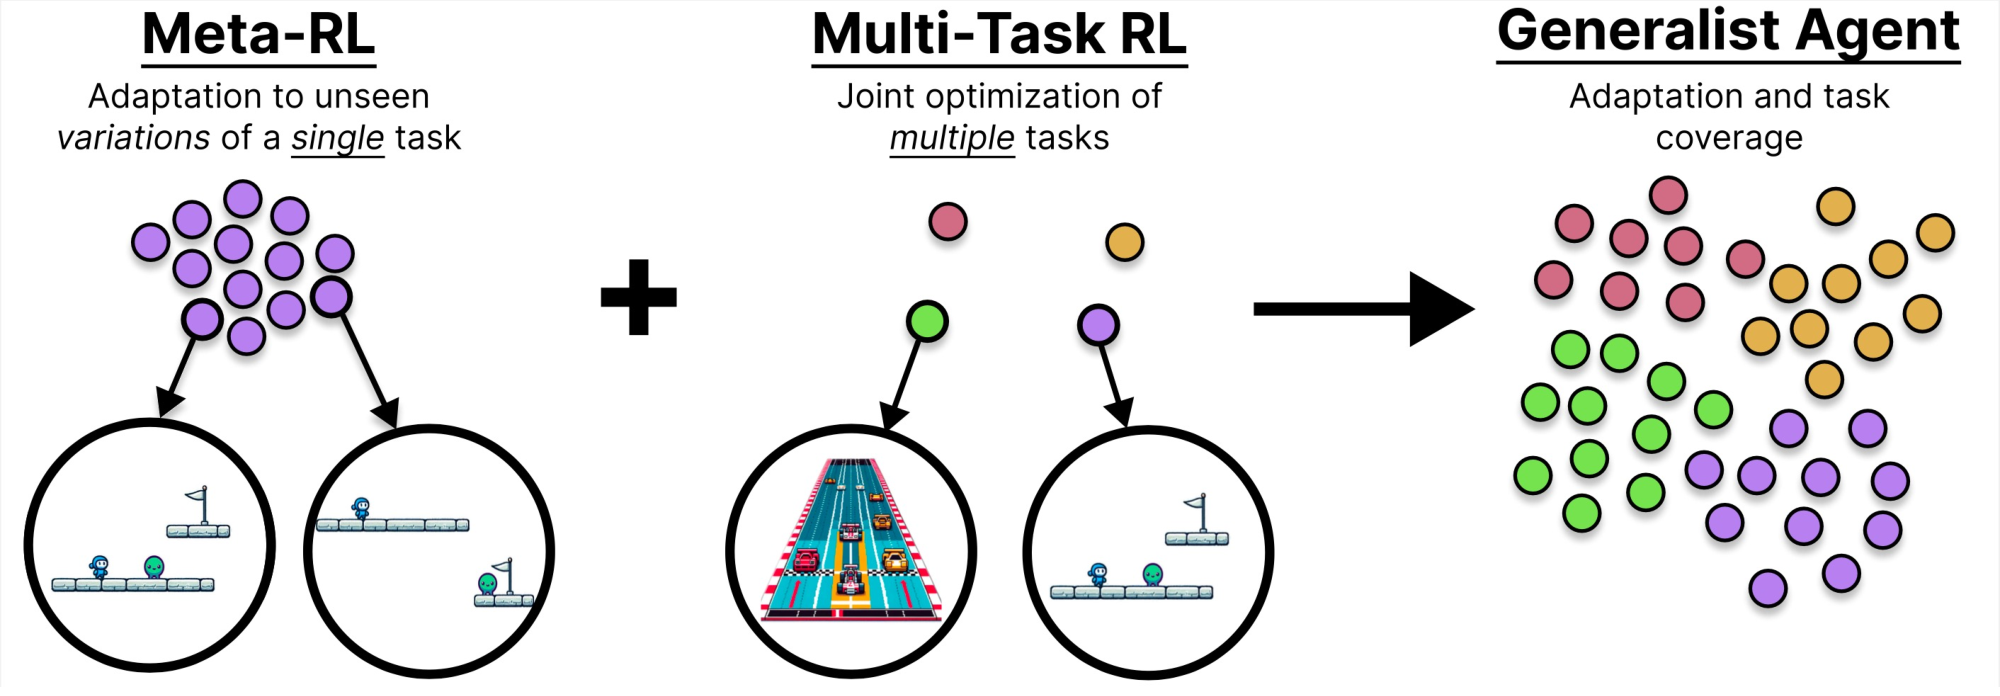
\includegraphics[width=.95\textwidth]{figures/final/fig1_v2_rerendered.pdf}
    \caption{\textbf{Task Spaces in RL Generalization.} Meta-RL agentso adapt to dense variations of a core task. Multi-Task RL overcomes optimization challenges of learning from isolated tasks. Scalable ideas from both areas allow us to extend adaptive agents towards increasingly general behavior.\vspace{-4mm}}
    \label{fig:fig1}
\end{figure}

Online Reinforcement Learning (RL) lets models continuously self-improve and directly optimizes performance. The RL equivalent of in-context learning is a subset of meta-RL techniques that use sequence models for memory and adaptation \cite{beck2023survey, wang2016learning, duan2016rl}. Meta-RL can be viewed as a \textit{task inference} problem in which an agent explores its new surroundings to discover information that it can use to improve decision-making \cite{humplik2019meta, ghosh2021generalization, zintgraf2022fast}. In theory, meta-RL can adapt to a wide range of control problems. However, current applications are quite narrow ---  usually focusing on minor variations of what could be considered a single task. For example, imagine a platformer video game with procedurally generated levels. The game has a consistent theme and controls, but each level introduces a slightly different reward function, physics, and layout. A meta-learning policy trained on this game would learn to identify the relevant changes in a new level in order to maximize returns. By most formal definitions, any two levels from this game would be considered two different ``tasks,'' but it seems unlikely that anyone outside the field would refer to the resulting policy as a ``multi-task" agent. A truly general agent would also be able to play entirely different games. We will use the term ``task" to refer to this kind of multi-game generality while calling different levels of the same game ``task \textit{variants}” \cite{zhao2022effectiveness, taiga2023investigating, rusu2022probing}. Each task (game) creates a distribution of variants (levels) we can sample. The distinction between two ``tasks'' and two ``variants'' of the same task is arbitrary in theory\footnote{The distinction between tasks/variants is also called non-parametric/parametric variation \cite{yu2020meta, lee2023parameterizing}. Variants are often generated by randomizing a known set of parameters in a single (simulated) environment.}. However, it is so relevant in practice that having separate terms will be important for clarity.

Ideally, we would train RL agents on many different tasks and many variants of those tasks. Recent works have scaled to heterogeneous mixtures of popular RL benchmarks \cite{reed2022a, hansen2023td, gallouedec2024jack}, but rely on offline datasets collected by expert single-task agents. Scaling up online learning is challenging because multi-task distributions can create disconnected datasets; as we transition from a single task to small sets of several tasks, we reach a barrier where the gap between tasks becomes so wide that practical optimization challenges hinder learning more than any knowledge transfer between them is helping \cite{taiga2023investigating, shaham2023causes, xin2022current}. This conflict is particularly limiting in meta-RL because multi-task behavior should otherwise be a simple case of task inference. Meta-RL agents learn to infer the identity of task variants based on limited information --- which becomes more challenging as those variants become more similar. Adding an entirely new task with clearly distinct visuals or controls does little to the difficulty of this problem, and yet it can dramatically reduce performance because it introduces the (mostly unrelated) challenge of optimizing a second reward function. Fortunately, this challenge is not unique to meta-RL and is a focus of broader research in multi-task RL (MTRL) and supervised learning \cite{zhang2021survey}. MTRL methods can improve multi-objective training by creating task-specific network parameters or editing the gradients of each task to resolve conflicting updates (Section \ref{sec:background}). Unfortunately, these solutions rely on our ability to manually label tasks, scale with the size of our training set, and can abandon meta-RL's goal of adapting to new tasks at test-time. While MTRL might be practical on current benchmarks, it would be more scalable to preserve meta-RL's task inference and improve multi-task optimization without introducing new assumptions (Figure \ref{fig:fig1}).


This paper focuses on training sequence model policies that generalize across hybrid task distributions containing elements of meta-RL, MTRL, and long-term memory. We revisit the idea that MTRL is primarily bottlenecked by imbalanced training losses created by tasks with returns on significantly different scales \cite{hessel2019multi}. However, we approach this problem from a meta-RL perspective where \textit{task inference needs to be learned; we do not allow knowledge of task labels to influence training in any way}. We experiment with Transformer \cite{vaswani2017attention} policies trained by mixtures of actor and critic objectives that are either directly or indirectly dependent on the scale of returns in any given task. Comparisons on Meta-World ML45 \cite{yu2020meta}, Multi-Task POPGym \cite{morad2023popgym}, Multi-Game Procgen \cite{cobbe2020leveraging}, Multi-Game Atari \cite{bellemare2013arcade}, and Multi-Task BabyAI \cite{chevalier-boisvert2018babyai} evaluate the importance of scale-resistant updates. We find that converting value regression to classification \cite{hafner2023mastering} and policy improvement to filtered imitation learning \cite{wang2020critic} leads to significant improvements in these hybrid settings. Our results suggest that scale invariance should be a priority when designing multi-task agents with adaptive memory. Our empirical success with classification updates further supports recent observations that sequence-based RL can improve by borrowing technical details from supervised sequence modeling \cite{chebotar2023q, farebrother2024stop, springenberg2024offline} while retaining the online self-improvement process that makes RL useful \cite{chen2021decision, lee2022multi}.

